%\newcommand{\ein}[2]{(#1) (#2 Punkte)}


\begin{Large}
\textbf{Teil I: Offene Aufgaben (40 Punkte)}
\end{Large}
\\
\\
\\
\textbf{Allgemeine Anweisungen für offene Fragen:}
\\
\renewcommand{\labelenumi}{(\roman{enumi})}
\begin{enumerate}
\item
Ihre Antworten müssen alle Rechenschritte enthalten,
diese müssen klar ersichtlich sein.
Verwendung korrekter mathematischer Notation wird erwartet
und fliesst in die Bewertung ein.

\item
Ihre Antworten zu den jeweiligen Teilaufgaben müssen in den dafür vorgesehenen Platz geschrie-
ben werden. Sollte dieser Platz nicht ausreichen, setzen Sie Ihre Antwort auf der Rückseite oder
dem separat zur Verfügung gestellten Papier fort. Verweisen Sie in solchen Fällen ausdrücklich
auf Ihre Fortsetzung. Bitte schreiben Sie zudem Ihren Vor- und Nachnamen auf jeden separaten
Lösungsbogen.

\item
Es werden nur Antworten im dafür vorgesehenen Platz bewertet. Antworten auf der Rückseite
oder separatem Papier werden nur bei einem vorhandenen und klaren Verweis darauf bewertet.

\item
Die Teilaufgaben werden mit den jeweils oben auf der Seite angegebenen Punkten bewertet.

\item
Ihre endgültige Lösung jeder Teilaufgabe darf nur eine einzige Version enthalten.

\item
Zwischenrechnungen und Notizen müssen auf einem getrennten Blatt gemacht werden. Diese
Blätter müssen, deutlich als Entwurf gekennzeichnet, ebenfalls abgegeben werden.
\end{enumerate}

\newpage
\section*{\hfil Aufgaben \hfil}
\vspace{1cm}
\section*{Aufgabe 1 (40 Punkte)}
\vspace{0.4cm}
Ein institutioneller Anleger beabsichtigt im großen Stil Aktien einer Firma zu kaufen.
Da der Handelspreis der Aktie jedoch von der Nachfrage abhängt, möchte der Investor zuerst verstehen, wie seine Nachfrage den Preis beeinflussen wird.
Die Nachfrage des Investors in Abhängigkeit vom Preis ist gegeben durch $ d = D(p) =4 - 2 e^{p-1}$.
Der Preis der Aktie in Abhängigkeit von der Nachfrage $ d $ des Investors ist gegeben durch $ P(d) = \frac{1}{4} + \frac{1}{2} d $.
%\titleformat{\subsection}[runin]
%{\normalfont\large\bfseries}{\thesubsection}{1em}{}
\subsection*{\aufgabe{a1}{2}} 
Verknüpfen Sie die beiden Funktionen $ P $ und $ D $ \hspace{\parindent}zur Funktion $ Q = P \circ D $,
\begin{align*}
	Q : R_+ \to \R_{++} , \ p \mapsto q= Q(p),
\end{align*}
welche die Beziehung zwischen dem neuen Preis $ q $ und dem alten Preis $ p $ beschreibt, nachdem 
der Investor $ D(p) $ Stück Aktien gekauft hat.
Geben Sie die Abbildungsvorschrift $ Q $ an.
\\
\\


\subsection*{\aufgabe{a2}{6}} Zeigen Sie, dass es einen eindeutigen Fixpunkt $ p^\star \in \left[0,\frac{3}{2}\right] $ gibt, für welchen die Relation $ p^\star = Q(p^\star) $ gilt.
Gesucht ist also der Gleichgewichtspreis $ p^\star $, welcher unverändert bleibt, wenn der Investor $ D(p^\star ) $ Stück Aktien kauft.
 \\
\\
\titleformat{\subsection}[display]
{\normalfont\large\bfseries}{\thesubsection}{1mm}{}
\subsection*{\aufgabe{a3}{6}}
Ein institutioneller Anleger beabsichtigt im großen Stil Aktien einer Firma zu kaufen.
Da der Handelspreis der Aktie jedoch von der Nachfrage abhängt, möchte der Investor zuerst verstehen, wie seine Nachfrage den Preis beeinflussen wird.
Die Nachfrage des Investors in Abhängigkeit vom Preis ist gegeben durch $ d = D(p) =4 - 2 e^{p-1}$.
Der Preis der Aktie in Abhängigkeit von der Nachfrage $ d $ des Investors ist gegeben durch $ P(d) = \frac{1}{4} + \frac{1}{2} d $.\\
Für die Funktion $ Q = P \circ D $ gibt es einen eindeutigen Punkt $ p^\star \in \left[0,\frac{3}{2}\right]  $ mit $ p^\star = Q(p^\star) $.\\
Verwenden Sie eine Taylor-Approximation zweiter Ordnung im Punkt $ p_0 = 1 $, um eine Näherung für $ p^\star  $ zu finden.
\\ \\
\subsection*{\aufgabe{b}{6}}
Ein Computer hat eine Rechenleistung von $ a_n $ während der Periode $ n, \ n = 1,2,... $
Mithilfe maschinellen Lernens erhöht sich die Rechenleistung in jeder Periode um $ 2 \%  $, wobei sie zu Beginn $ a_1 = 10 $ beträgt.
Mit dem Computer benötigt die vollständige Berechnung einer bestimmten, anspruchsvollen Aufgabe $ 15 $ Perioden (d.h. die komplette Rechenleistung der ersten 15 Perioden wird für die Berechnung benötigt).\\
Anstelle die Berechnungen direkt zu starten, beschliesst das Rechenzentrum  zunächst die Rechenleistung des Computers aufzustocken.
Damit kann mit der Aufgabe zwar erst nach $ 3 $ Perioden begonnen werden, dafür aber hat der Computer nun eine neue anfängliche Rechenleistung von $ 15 $, welche sich pro Periode um $ 3 \% $ erhöht.\\
Wie viel Zeit (in Perioden) kann das Rechenzentrum durch das Aufstocken des Computers und den Aufschub der Berechnung einsparen?
\\ 
\\
\subsection*{\aufgabe{c}{10}}
Eine Familie leiht sich CHF $ 1'000'000 $, um ein Haus zu kaufen.
Der Zins beträgt zu Beginn $ i = 1 \% $.
Die Familie beschliesst, CHF $ C_1 $ am Ende jeden Jahres für $ 10 $ Jahre zurückzuzahlen, um so den Schuldenstand auf CHF $ 750'000 $ am Ende des $ 10. $ Jahres zu reduzieren.
Am Ende des $ 5 $-ten Jahres ergibt sich die Möglichkeit einer Sondertilgung.
Die Familie zahlt folglich am Ende des $ 5 $-ten Jahres einen Gesamtbetrag von CHF $ 150'000 $ (einschliesslich $ C_1 $) zurück und verhandelt die Konditionen mit der Bank neu.
Der Zinssatz fällt damit auf $ 0.5 \% $.
Die Familie beschliesst, die Schulden weiterhin mit CHF $ C_1 $ am Ende jeden Jahres zurückzuzahlen, bis diese auf CHF $ 500'000 $ reduziert sind.
Aus steuerlichen Gründen zahlen sie anschliessend CHF $ C_2 $ pro Jahr an die Bank,
um ihre Schulden konstant bei CHF $ 500'000 $ zu halten.
\begin{enumerate}
	\item[(c1)]
	Fügen Sie alle Ereignisse und Mittelflüsse dem Zeitstrahl hinzu.
	\item[(c2)] 
	Berechnen Sie $ C_1 $.
	\item[(c3)] Wie hoch ist der Schuldenstand, nachdem die Familie die Zahlung von CHF 150'000 am Ende des $ 5 $-ten Jahres veranlasst hat?
	\item[(c4)] 
	Wie lange dauert es nach Ende des $ 5 $-ten Jahres, bis der Schuldenstand CHF $ 500'000 $ erreicht hat?
	\item[(c5)]
	Berechnen Sie $ C_2 $.
\end{enumerate}
\begin{center}
	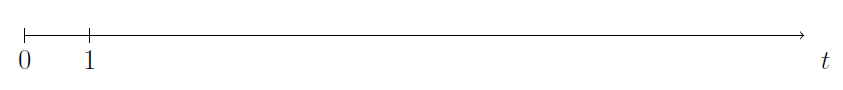
\includegraphics[scale=0.6]{pictures/zeitstrahl_1_c}
\end{center}

\newpage

\subsection*{\aufgabe{d}{10}}
Ein Anbieter für Tablets schätzt die Nachfrage $ q_d $ nach seinem neusten Produkt auf
\begin{align*}
	q_d(p)
	=
	\frac{15'840 - 30 \ p}{p + 50},
\end{align*}
wobei $ p > 20  $ der Verkaufspreis in US-Dollar pro Tablet ist.
Die Kosten für Produktion und Vertrieb eines Tablets betragen $ 20  $ US-Dollar.
\begin{enumerate}
	\item[(d1)]
	Bestimmen Sie die Gewinnfunktion des Anbieters unter der Annahme, dass der Preis $ p > 20 $ ist.
	\item[(d2)]
	Leiten Sie die Funktion her, welche die Elastizität des Gewinns in Abhängigkeit vom Verkaufspreis beschreibt.
	\item[(d3)]
	Approximieren Sie mit Hilfe der Elastizitätsfunktion die relative Änderung des Gewinns bei einer Erhöhung des anfänglichen Verkaufspreises von $ p_0 = 100 $ US-Dollar um $ 5 $ US-Dollar.
\end{enumerate}

\newpage


\fancyhead[C]{\normalsize\textbf{$\qquad$ Teil II: Multiple-Choice}}
\begin{Large}
\textbf{Teil II: Multiple-Choice-Fragen (60 Punkte)}
\end{Large}
\\
\\
\\
\textbf{Allgemeine Anweisungen für Multiple-Choice-Fragen:}
\\
\renewcommand{\labelenumi}{(\roman{enumi})}
\begin{enumerate}
\item
Die Antworten auf die Multiple-Choice-Fragen müssen im dafür vorgesehenen Antwortbogen ein-
getragen werden. Es werden ausschliesslich Antworten auf diesem Antwortbogen bewertet. Der
Platz unter den Fragen ist nur für Notizen vorgesehen und wird nicht korrigiert.

\item
Jede Frage hat nur eine richtige Antwort. Es muss also auch jeweils nur eine Antwort angekreuzt
werden.

\item
Falls mehrere Antworten angekreuzt sind, wird die Antwort mit 0 Punkten bewertet, auch wenn
die korrekte Antwort unter den angekreuzten ist.

\item
Bitte lesen Sie die Fragen sorgfältig.

\end{enumerate}
\newpage
\section*{Aufgabe 2 (32 Punkte)}
\vspace{0.4cm}

\subsection*{\frage{1}{4}}
Welche der folgenden Aussagen ist wahr, genau dann wenn $ A $ und $ B $ in ihrem Wahrheitsgehalt verschieden sind (eine Aussage ist wahr, die andere falsch)?
 \renewcommand{\labelenumi}{(\alph{enumi})}
\begin{enumerate}
\item $ A \vee B $.
\item $ A \wedge B $.
\item $ \neg (A \Rightarrow B) $.
\item $ (A \vee B) \wedge (\not(A \wedge B)) $.
\end{enumerate}
\ \\
\subsection*{\frage{2}{3}}
Sei $ A = \textrm{\glqq Jeanette und Hans kommen an die Party \grqq} $
und $ B = \textrm{\glqq Mark kommt an die Party \grqq}  $.
Wir wissen, dass Hans die Party nicht besuchte.
Über Jeanette und Mark ist jedoch nichts bekannt.\\
Welche Aussage ist demnach richtig?
\renewcommand{\labelenumi}{(\alph{enumi})}
\begin{enumerate}
\item $ A \wedge B $.
\item $ A \vee B $.
\item $ A \Rightarrow B $.
\item $ A \Leftrightarrow B $.
\end{enumerate}
\ \\
\subsection*{\frage{3}{3}}
Die Folge $ \{ a_n \}_{n \in \N} $ ist beschränkt, monoton und konvergent.
Zudem gilt $ a_n \neq 0  $ für alle $ n $.
Sei $ \{b_n\}_{n \in \N} $ die Folge definiert durch $ b_n = \frac{1}{a_n} $.
Dann folgt:
\renewcommand{\labelenumi}{(\alph{enumi})}
\begin{enumerate}
\item 
$ \{b_n \}_{n \in \N} $ ist beschränkt.
\item 
$ \{b_n\}_{n \in \N} $ ist monoton.
\item 
$ \{b_n\}_{n \in \N} $ ist konvergent.
\item
Keine der obigen Eigenschaften folgt.
\end{enumerate}
\ \\
\subsection*{\frage{4}{4}}
Sei $ \{ a_n \}_{n \in \N} $ eine geometrische Folge mit 
$ \frac{a_{n+1}}{a_n} = q \in (0,1) $.
Sei $ \{ b_n \}_{n \in \N} $ eine andere geometrische Folge mit
$ \frac{b_{n+1}}{b_n} = \frac{q}{2} $.\\
Zudem gilt: $ \sum_{k = 1}^\infty a_k = \sum_{k = 1}^\infty b_k $.
Dann folgt
\renewcommand{\labelenumi}{(\alph{enumi})}
\begin{enumerate}
	\item 
	$ b_1 = 2 a_1 $, falls $ q = \frac{1}{3} $.
	\item
	$ b_1 = 2 a_1 $, falls $ q = \frac{1}{2} $.
	\item
	$ b_1 = 2 a_1 $, falls $ q = \frac{2}{3} $.
	\item
	Die Bedingung $ b_1 = 2 a_1 $ ist nie erfüllt.
\end{enumerate}
\ \\
\subsection*{\frage{5}{3}}
Am Tag, an dem Mark einen Kredit über $ P_1= 1'000'000 $ CHF mit Zinssatz $ i_1 = 1 \% $ aufnimmt, nimmt Lucie einen Kredit über $ P_2= 800'000 $ CHF mit Zinssatz $ i_2 = 1.2 \% $ auf.
Mark zahlt den Kredit in konstanten Raten von $ 10'500 $ CHF jeweils am Ende des Jahres zurück, während Lucie $ 9'500 $ CHF auch jeweils am Ende des Jahres zurückbezahlt.\\
Welche der folgenden Antworten ist richtig?
\renewcommand{\labelenumi}{(\alph{enumi})}
\begin{enumerate}
	\item 
	Mark bezahlt den Kredit vor Lucie zurück.
	\item 
	Lucie bezahlt den Kredit vor Mark zurück.
	\item
	Lucie und Mark bezahlen den Kredit zum gleichen Zeitpunkt zurück.
	\item
	Keine der obigen Antworten ist richtig..
\end{enumerate}
\ \\
\subsection*{\frage{6}{3}}
Seien $ f $ und $ g $ Funktionen einer reellen Variable mit Definitionsbereich $ D_f $ beziehungsweise $ D_g $.\\
Sei $ h = f \circ g $.
Welche der folgenden Aussagen über den Definitionsbereich $ D_h $ ist richtig?
\renewcommand{\labelenumi}{(\alph{enumi})}
\begin{enumerate}
	\item 
	$ D_h = D_f \cup D_g$.
	\item 
	$ D_h \subseteq D_g $.
	\item
	$ D_h \subseteq D_f $.
	\item
	$ D_h = D_f \cap  D_g $.
\end{enumerate}
\ \\
\subsection*{\frage{7}{3}}
Eine Funktion $ f $ mit Definitionsbereich $ D_f \subseteq \R_{++} $ habe eine Elastizität $ \varepsilon_f $, die konstant gleich $ 2 $ ist.\\
\\
Welche der folgenden Aussagen über die die Wachstumsrate $ \rho_f $ von $ f $ ist richtig?
\renewcommand{\labelenumi}{(\alph{enumi})}
\begin{enumerate}
\item 
$ \rho_f $ ist streng monoton fallend.
\item
$ \rho_f $ ist streng monoton wachsend.
\item
$ \rho_f $ ist konstant.
\item
$ \rho_f $ ist nicht monoton.
\end{enumerate}
\ \\
\subsection*{\frage{8}{4}}
Eine differenzierbare Funktion $ f : D_f \to \R  $ ist streng konkav und erfüllt $ f(x)  > 0 $ für alle $ x \in D_f $.
Zudem gibt es ein $ x_0 \in D_f, x_0 \neq 0 $, so dass für die Elastizität von $ f $ an der Stelle $ \varepsilon_f(x_0 ) = 0 $ gilt.\\
Welche der folgenden Aussagen ist richtig?
\renewcommand{\labelenumi}{(\alph{enumi})}
\begin{enumerate}
	\item 
	Bei $ x_0 $ ist $ f $ elastisch.
	\item
	Bei $ x_0 $ besitzt $ f $ ein lokales Minimum.
	
	
	\item
	Bei $ x_0 $ besitzt $ f $ ein lokales Maximum.
	\item
	Keine der obigen Antworten ist richtig.
\end{enumerate}
\ \\
\subsection*{\frage{9}{3}}
Sei $ f $ eine Funktion einer reellen Variable, die mindestens $ n $-mal differenzierbar ist.
Sei $ P_k $ das Taylor-Polynom $ k $-ter Ordnung von $ f $ an der Stelle $ x_0 $, für $ k = 1,...,n-1 $, und $ R_k $ das zugehörige Restglied $ k $-ter Ordnung.\\
Welche der folgenden Aussagen ist richtig? 
\renewcommand{\labelenumi}{(\alph{enumi})}
\begin{enumerate}
	\item 
	Für alle $ x \in D_f $ und $  k = 2,...,n-1 $ gilt,
	dass $ R_k(x) < R_{k-1}(x) $.
	\item
	Für alle $ x \in D_f $ und $  k = 2,...,n-1 $ gilt,
	dass $ R_k(x) > R_{k-1}(x) $.
	
	\item
	Für alle $ x \in D_f $ und $  k = 2,...,n-1 $ gilt,
	dass $ R_k(x) = R_{k-1}(x) $.
	\item
	Keine der obigen Aussagen ist richtig.
\end{enumerate}
\ \\
\subsection*{\frage{10}{2}}
Eine Funktion zweier reellen Variablen $ f $ sei homogen von Grad $ 2 $ und ihre partielle Elastizität erfülle 
\begin{align*}
	\varepsilon_{f,y}(x,y) = e^{x+y} +1. 
\end{align*}
Dann folgt:
\renewcommand{\labelenumi}{(\alph{enumi})}
\begin{enumerate}
	\item 
	$ 	\varepsilon_{f,x}(x,y)  = 1 + e^{x+y}$.
	\item
	$ 	\varepsilon_{f,x}(x,y)  = 1 - e^{x+y}$.
	
	\item
	$ 	\varepsilon_{f,x}(x,y)  =  e^{x+y}$.
	\item
	$ 	\varepsilon_{f,x}(x,y)  = - e^{x+y}$.
\end{enumerate}
\newpage
\section*{Aufgabe 3 (28 Punkte)}
\vspace{0.4cm}

\subsection*{\frage{1}{4}}
Der rechtsseitige Grenzwert
\begin{align*}
	\lim\limits_{x \to 1 +}
	\left(
	\frac{1}{x-1} - \frac{1}{\ln(x)}
	\right)
\end{align*}
ist gleich:
\renewcommand{\labelenumi}{(\alph{enumi})}
\begin{enumerate}
\item 
$ -\frac{1}{2}$.
\item
$ 0$.
\item
$ \frac{1}{2}$.
\item
$ \infty$.
\end{enumerate}
\ \\
\subsection*{\frage{2}{4}}
Der rechtsseitige Grenzwert
\begin{align*}
	\lim\limits_{x \to 0 +}
	x^x
\end{align*}
ist gleich:
\renewcommand{\labelenumi}{(\alph{enumi})}
\begin{enumerate}
	\item 
	$0$.
	\item
	$1$.
	\item
	$e$.
	\item
	$e^e$.	
\end{enumerate}
\ \\
\subsection*{\frage{3}{4}}
Ein Blatt Papier sei $ 0.5 $ Millimeter dick. Man faltet das Blatt nun in der Hälfte, so dass es eine neue Dicke von $ 1 $ Millimeter hat.
Anschliessend faltet man es solange erneut, bis die Dicke des gefalteten Papiers $ 400'000 $ Kilometer erreicht (ungefähr die Distanz zwischen Erde und Mond).\\
Wie oft muss das Blatt Papier gefaltet werden ? 
\renewcommand{\labelenumi}{(\alph{enumi})}
\begin{enumerate}
\item 
Ungefähr $ 20 $ Mal.
\item
Ungefähr $ 30 $ Mal.
\item
Ungefähr $ 40 $ Mal.
\item
Ungefähr $ 50 $ Mal.
\end{enumerate}
\ \\
\subsection*{\frage{4}{4}}
Ein Projekt benötigt eine Anfangsinvestition von $ 10'000 $ CHF.
Nach einem Jahr generiert das Projekt eine Auszahlung in Höhe von $ 5'000  $ CHF und nach zwei Jahren eine Auszahlung in Höhe von $ 10'000 $ CHF.\\
Der interne Zinssatz des Projekts ist ungefähr
\renewcommand{\labelenumi}{(\alph{enumi})}
\begin{enumerate}
\item 
$ 5 \% $.
\item 
$ 10 \% $.
\item
$ 20 \% $.
\item
$ 30 \% $.
\end{enumerate}
\ \\
\subsection*{\frage{5}{3}}
Gegeben sei die Funktion $ f :D_f \to \R, (x,y) \mapsto z = f(x,y) = \frac{\ln(x^2 +y^2 -1)}{\sqrt{4 - x^2 - y^2}} $.
\renewcommand{\labelenumi}{(\alph{enumi})}
\begin{enumerate}
\item 
Der Definitionsbereich von $ f  $ ist das Innere (ohne Rand) des Kreises mit Mittelpunkt $ (0,0) $ und Radius $ 1 $.
\item
Der Definitionsbereich von $ f  $ ist das Innere (ohne Rand) des Kreises mit Mittelpunkt $ (0,0) $ und Radius $ 2 $.
\item
Der Definitionsbereich von $ f  $ ist das Innere (ohne Rand) des Kreises mit Mittelpunkt $ (0,0) $ und Radius $ 2 $, ohne das Innere (mit Rand) des Kreises mit Mittelpunkt $ (0,0) $ und Radius $ 1 $.
\item
Der Definitionsbereich von $ f  $ ist die leere Menge.
\end{enumerate}
\ \\
\subsection*{\frage{6}{3}}
Sei $ f $ eine Funktion zweier reellen Variablen gegeben durch:
\begin{align*}
	f: \R_{++}^2 \to \R, \ (x,y) \mapsto z = f(x,y) = 10 x^\alpha y^{1- \alpha},
\end{align*}
wobei $ \alpha \in (0,1) $.\\
Die Steigung der Tangente an die Niveaulinie von $ f $ am Punkt $ (x_0,y_0) = (1,1) $ ist gleich $ -0.5 $.\\
Dann folgt:
\renewcommand{\labelenumi}{(\alph{enumi})}
\begin{enumerate}
	\item 
	$ \alpha = \frac{1}{6}$.
	\item
	$ \alpha = \frac{1}{3}$.
	\item
	$ \alpha = \frac{1}{2}$.
	\item
	$ \alpha = \frac{2}{3}$.
\end{enumerate}
\ \\
\subsection*{\frage{7}{3}}
Gegeben ist die Funktion
\begin{align*}
	f(x,y) 
	=
	\ln\left(
	x^3 \sqrt[3]{y^4} + \sqrt[6]{x^{11} y^{15}}
	\right)
	- \frac{13}{3} \ln(x) \quad \textrm{für } x>0,y>0.
\end{align*}
Welche der folgenden Aussagen ist richtig?
\renewcommand{\labelenumi}{(\alph{enumi})}
\begin{enumerate}
\item
$ f  $ ist homogen von Grad $ 5 $.
\item
$ f $ ist linear homogen.	
\item 
$ f  $ ist homogen von Grad $ 0 $.
\item
$ f $ ist nicht homogen.
\end{enumerate}
\ \\
\subsection*{\frage{8}{3}}
Sei $ f $ eine Funktion einer reellen Variablen, definiert als $ f(x) = x^\alpha $ für $ \alpha > 0 $, und sei $ g $ eine Funktion zweier reellen Variablen, die strikt positiv und homogen von Grad $ \kappa $ ist.\\
Wir definieren die Funktion $ h $ als $ h(x,y)  = f(g(x,y))$.\\
Welche der folgenden Aussagen ist richtig?
\renewcommand{\labelenumi}{(\alph{enumi})}
\begin{enumerate}
	\item 
	$ h $ ist homogen von Grad $ 1 $, falls $ \alpha =0.5 $ und $ \kappa = 1 $.
	\item
	$ h $ ist homogen von Grad $ 2 $, falls $ \alpha =0.5 $ und $ \kappa = 4 $.
	\item
	$ h $ ist homogen von Grad $ 3 $, falls $ \alpha =0.5 $ und $ \kappa = 7 $.
	\item
	$ h $ ist homogen von Grad $ 5 $, falls $ \alpha =0.5 $ und $ \kappa = 11 $.
\end{enumerate}